\chapter{Experimental Results}
\label{chap:results}

\section{Calibration}
The distance estimation from the Received Signal Strength Indicator (RSSI) is computed using \autoref{eq:BLE_RSSI}, which includes two meta-parameters. The first parameter, $tx_{power}$, represents the RSSI at a distance of one meter. The second parameter, the environmental factor ($N$), accounts for signal propagation characteristics that depend on the surroundings.

\subsection{RSSI at One Meter ($tx_{power}$)}
Results from the first experiment in \autoref{exp:1_accuracy} are displayed in \autoref{fig:beacon-rssi-1m}. These results indicate that although the RSSI distribution shows some variability, it remains centered around the mean. The optimal $tx_{power}$ values can be obtained by averaging the RSSI values for each beacon.

Empirical results are consistent with the expected theoretical value of $-69$. The first two beacons yield values very close to this reference, while the third beacon reports a slightly higher RSSI of $-63$. The broader distribution for this beacon may suggest environmental influences affecting signal strength.

\begin{figure}[h]
    \centering
    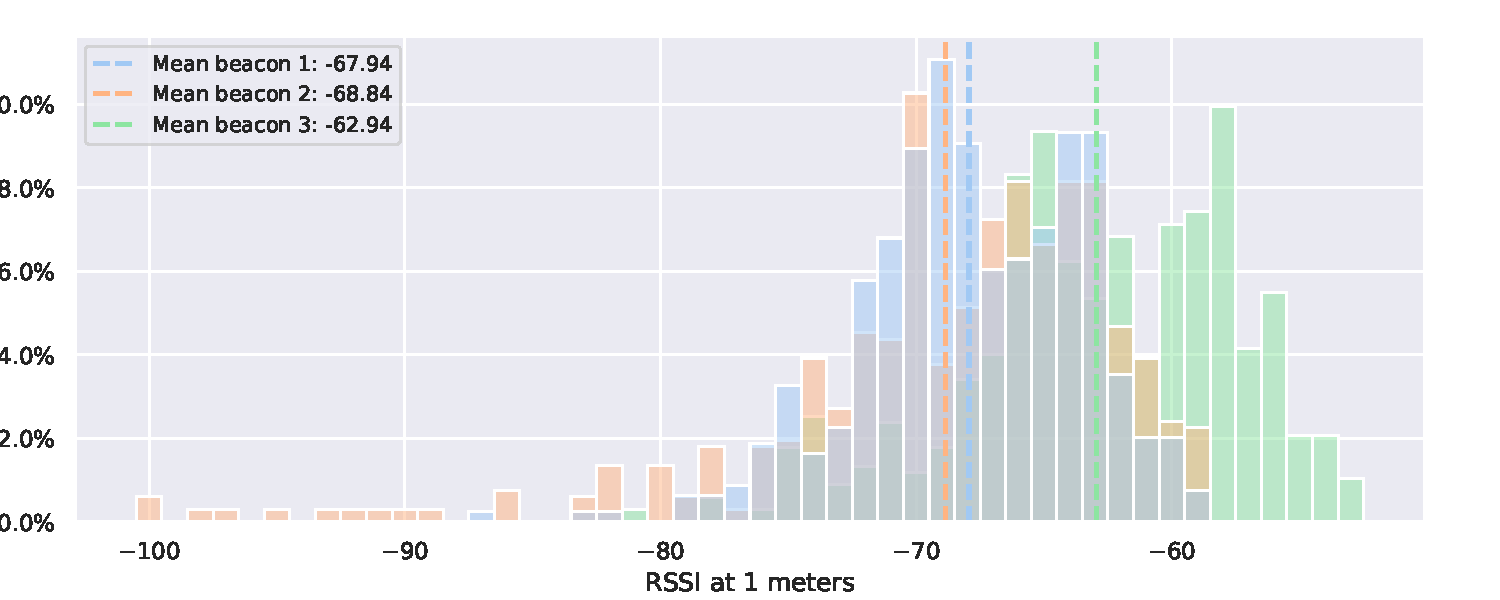
\includegraphics[width=\linewidth]{assets/beacon-rssi-1m.pdf}
    \caption{Experimental RSSI values at 1 meter}
    \label{fig:beacon-rssi-1m}
\end{figure}

\subsection{Environmental Factor ($N$)}
The environmental factor $N$ typically ranges from 2 in ideal conditions to 4 in highly obstructed or chaotic environments. Experimental results shown in \autoref{fig:beacon-environmental-factor} support this range. The plots illustrate the Mean Squared Error (MSE) between measured distances and those calculated using various values of $N$ (from 2 to 4), applied to measurements taken from both Experiment 1 (corridor) and Experiment 2 (museum).

In the corridor environment, which features line-of-sight (LoS) conditions and minimal interference, the optimal environmental factor is approximately 2.07. In contrast, measurements taken in the museum, with by complex layouts and significant obstructions, produce a higher MSE across all values of $N$. The lowest error occurs with $N = 2.83$, reflecting the increased signal attenuation due to environmental factors.

\begin{figure}[h]
    \centering
    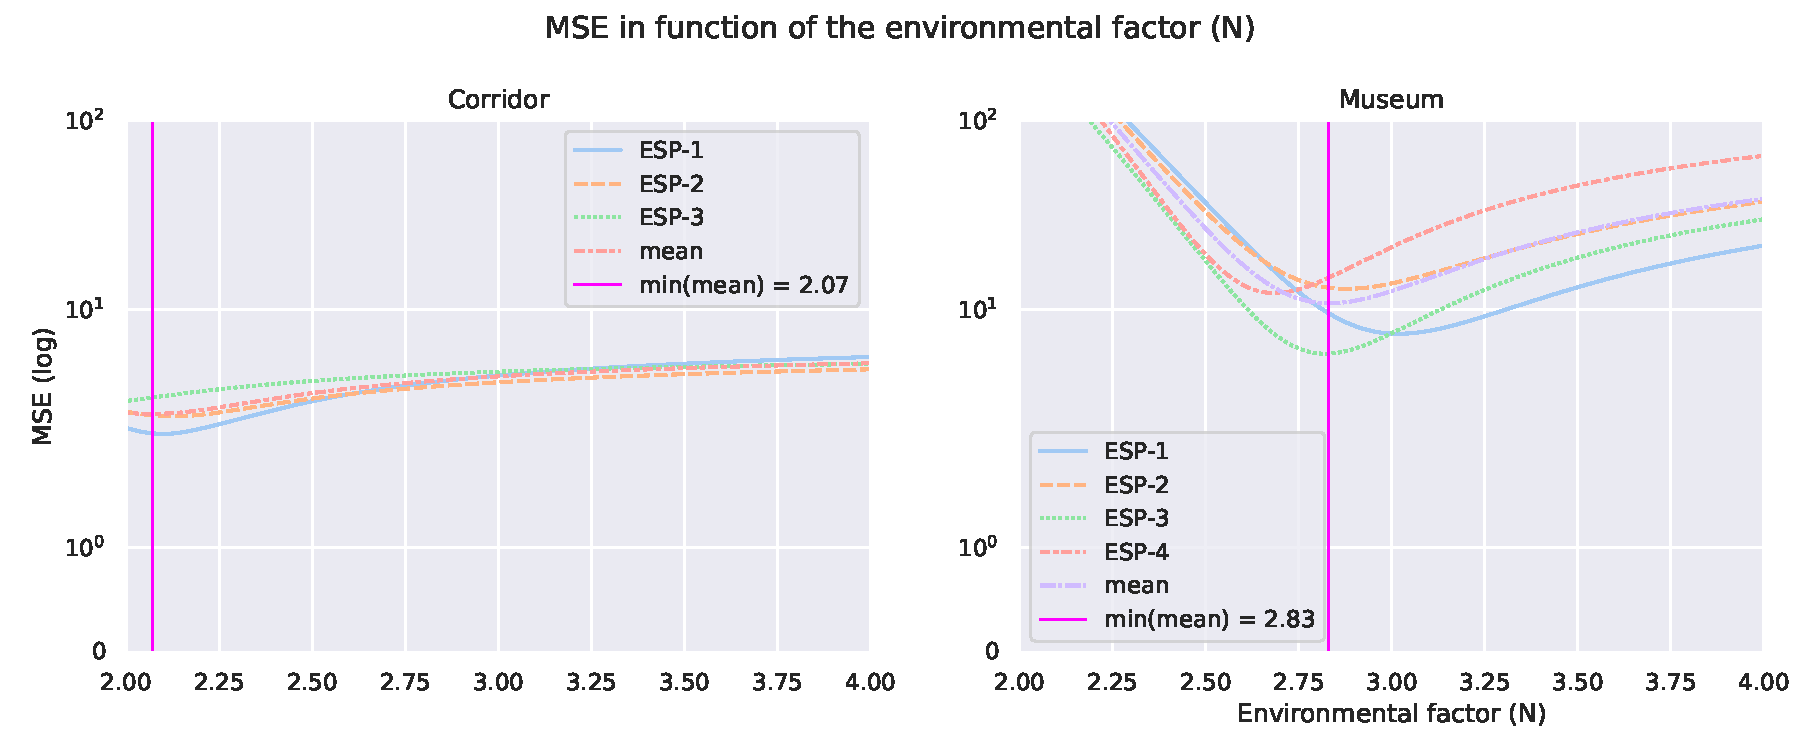
\includegraphics[width=\linewidth]{assets/beacons-environmental-factor.pdf}
    \caption{Comparison of environmental factors ($N$) in both test environments}
    \label{fig:beacon-environmental-factor}
\end{figure}

\subsection{Summary of Calibration Findings}

These findings confirm that the theoretical value of $tx_{power} = -69$ is robust and does not require adjustment based on environment. In contrast, the environmental factor $N$ must be calibrated for each new environment. Nevertheless, once determined, the same $N$ can be applied uniformly across all beacons, thus simplifying the setup process.

\section{Distance to Beacons}
Experimental data from Experiment 1, as shown in \autoref{fig:beacon-dist-raw-error}, confirm the findings reported by \cite{spachos_ble_2020}, which highlight a correlation between ranging precision and beacon distance. Specifically, beacons located within a few meters provide highly accurate distance estimates with minimal error spread.

\begin{figure}[h]
    \centering
    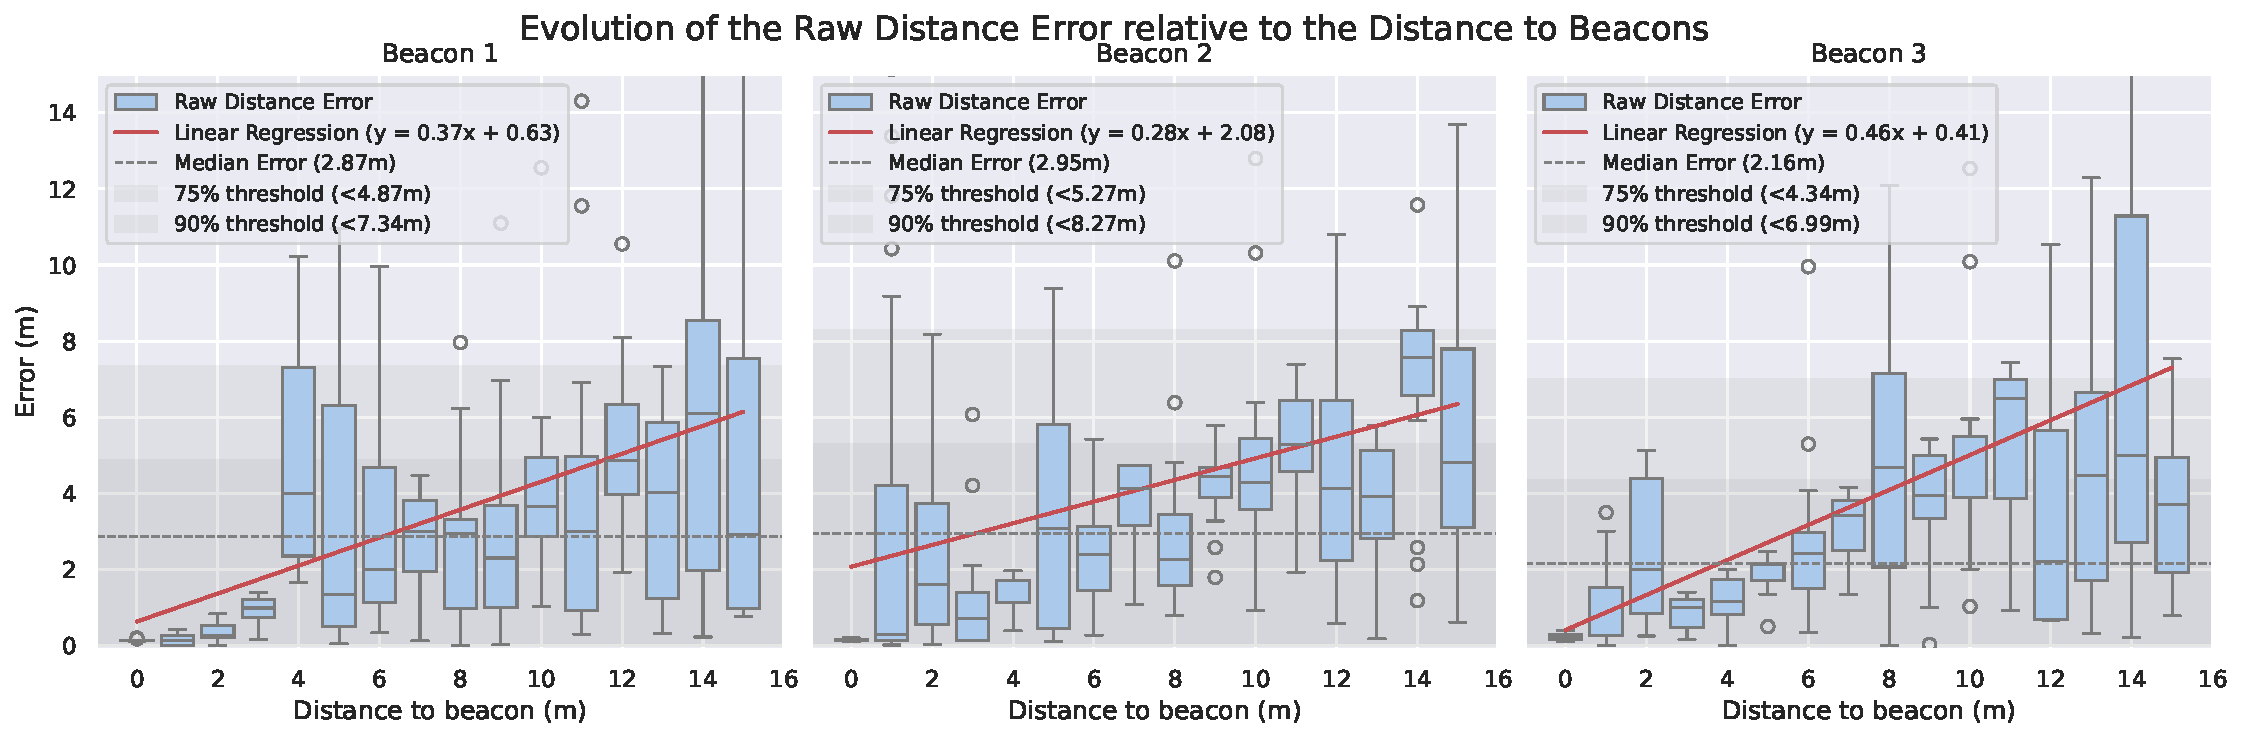
\includegraphics[width=\linewidth]{assets/beacon-dist-raw-error-by-beacon.pdf}
    \caption{Raw distance error variation relative to distance from beacons}
    \label{fig:beacon-dist-raw-error}
\end{figure}

Analysis of the raw distance errors shows that the median error typically lies between 2 and 3 meters. Moreover, 75\% of distance errors are below 5 meters, and 90\% fall below 8 meters.

After applying a Kalman filter to the data, as presented in \autoref{fig:beacon-dist-filtered-error}, error margins are significantly reduced. The median error decreases to between 1.5 and 2.5 meters, with 75\% of errors below 4 meters. However, the 90\% threshold remains around 8 meters, indicating that although the filter reduces overall noise, extreme conditions still lead to larger errors.

\begin{figure}[h]
    \centering
    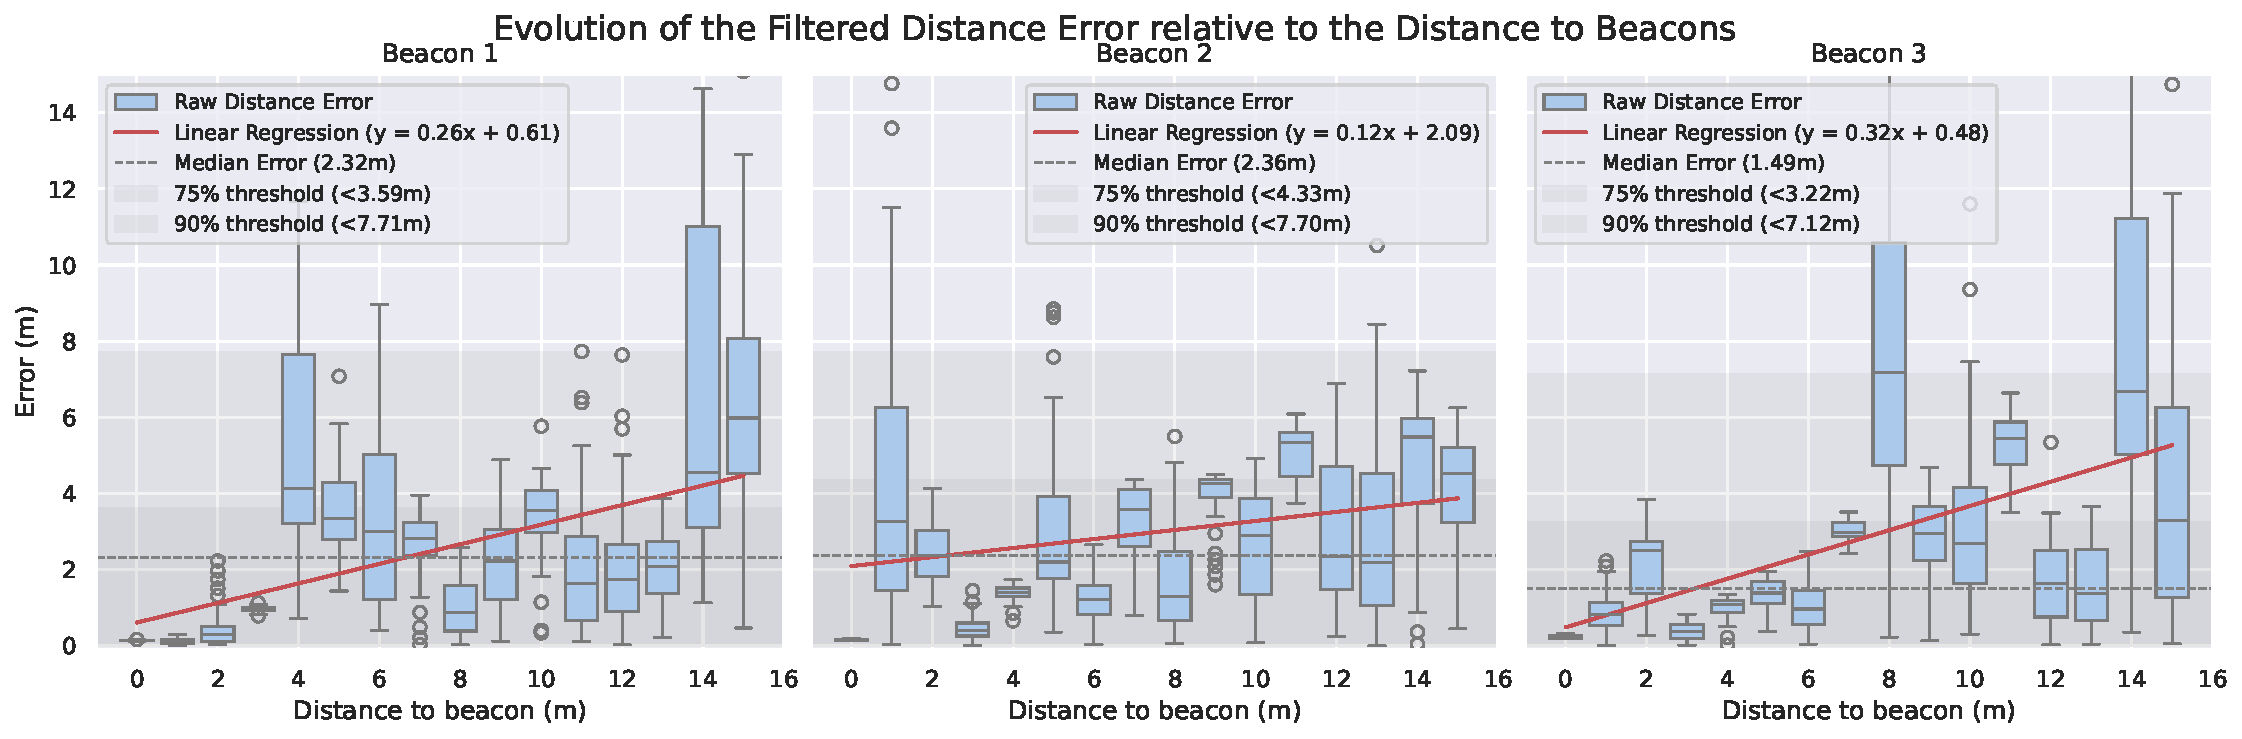
\includegraphics[width=\linewidth]{assets/beacon-dist-filtered-error-by-beacon.pdf}
    \caption{Filtered distance error variation relative to distance from beacons}
    \label{fig:beacon-dist-filtered-error}
\end{figure}

\section{Multi-lateration precision}

The multi-lateration algorithm was evaluated based on its ability to estimate the position of the smartphone relative to the BLE beacons. The results demonstrate that the system achieves a median localization error of 2.8 meters, as show by \autoref{fig:trilateration-raw-error}), indicating that, in typical conditions, the estimated position is within 2.8 meters of the actual location. Furthermore, the distribution of errors shows that 75\% of the position estimates fall within 3.86 meters, and 90\% are within 5.81 meters. These results highlight the robustness of the multi-lateration approach in the tested environment, even in the presence of signal fluctuations and environmental noise.

\begin{figure}[H]
		\centering
		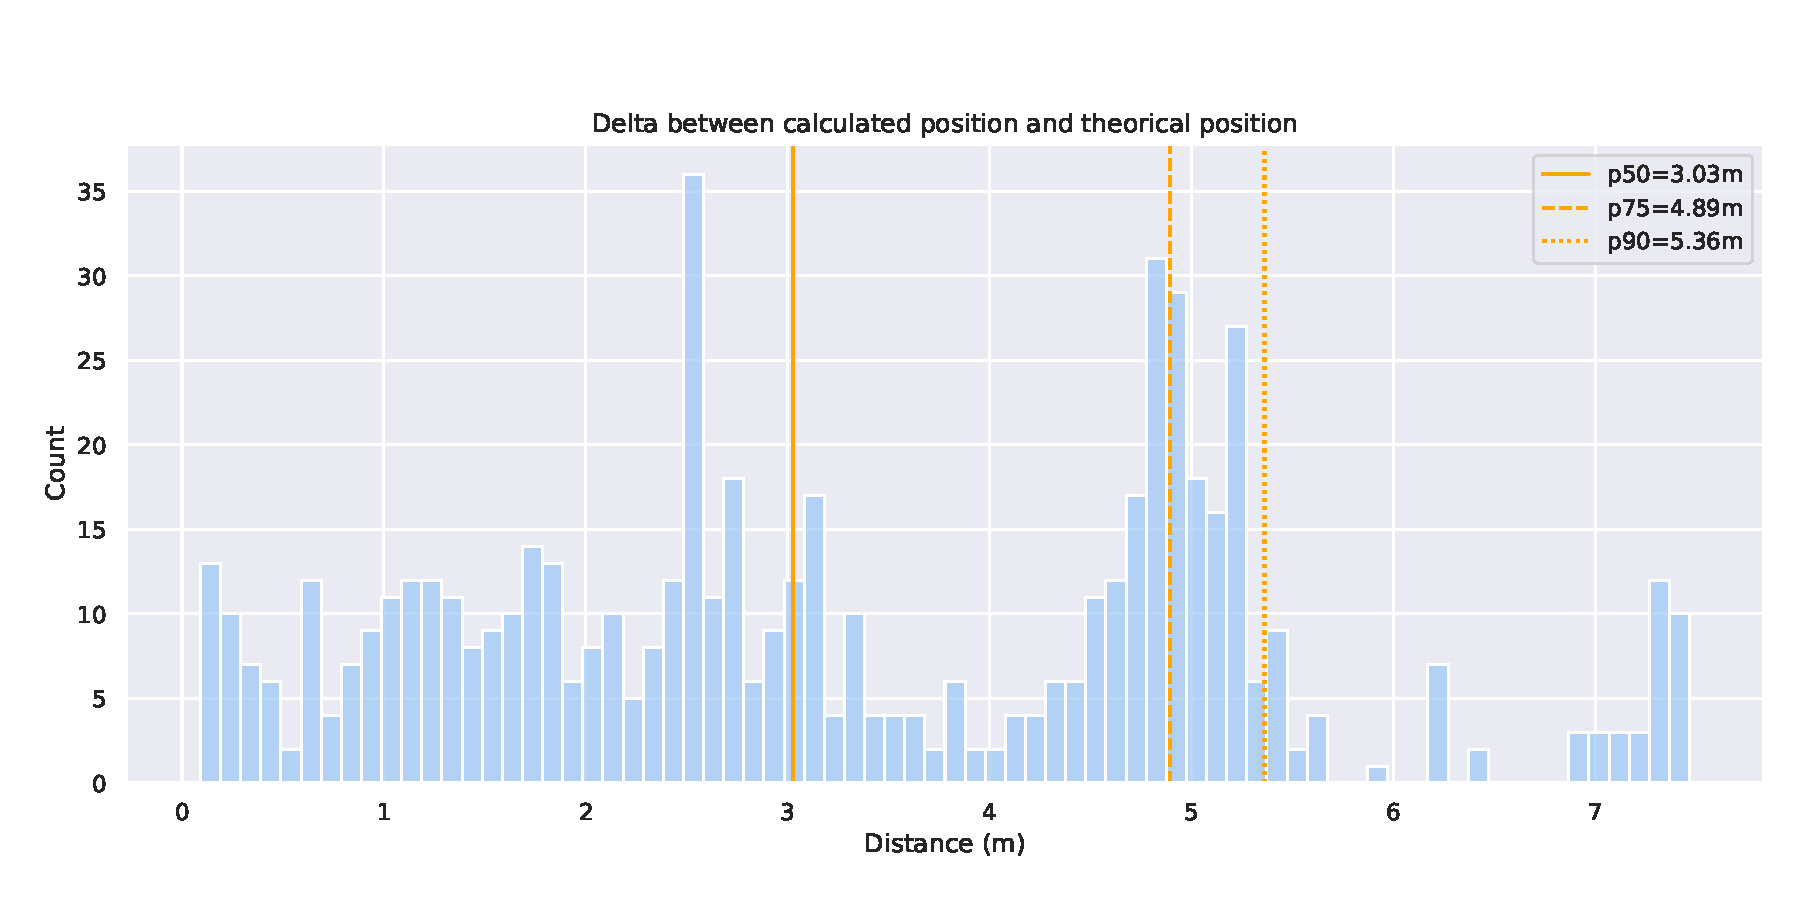
\includegraphics[width=\linewidth]{assets/museum-location-precision.pdf}
		\caption{Multi-lateration error in the museum environment}
		\label{fig:trilateration-raw-error}
\end{figure}


It is important to note that in 9\% of the measurements, the system was unable to compute a position estimate. This was primarily due to insufficient data, such as a lack of simultaneous beacon signals required for multi-lateration. While this represents a small fraction of the total measurements, it underscores the importance of beacon placement and signal coverage in ensuring continuous localization. Overall, the multi-lateration method provided reliable and reasonably accurate position estimates for the majority of the experiment duration.


\section{Area detection}

As shown in \autoref{fig:area-precision}, the correct area is detected in more than 80\% of cases. However, the detection accuracy varies significantly depending on the specific area. Side areas (steps 1, 2, 3, 5, and 6) achieve near-perfect detection rates, ranging from 93\% to 100\%. In contrast, central areas (steps 0 and 4) are correctly identified in only 27\% and 57\% of the cases, respectively.

\begin{figure}[h]
		\centering
		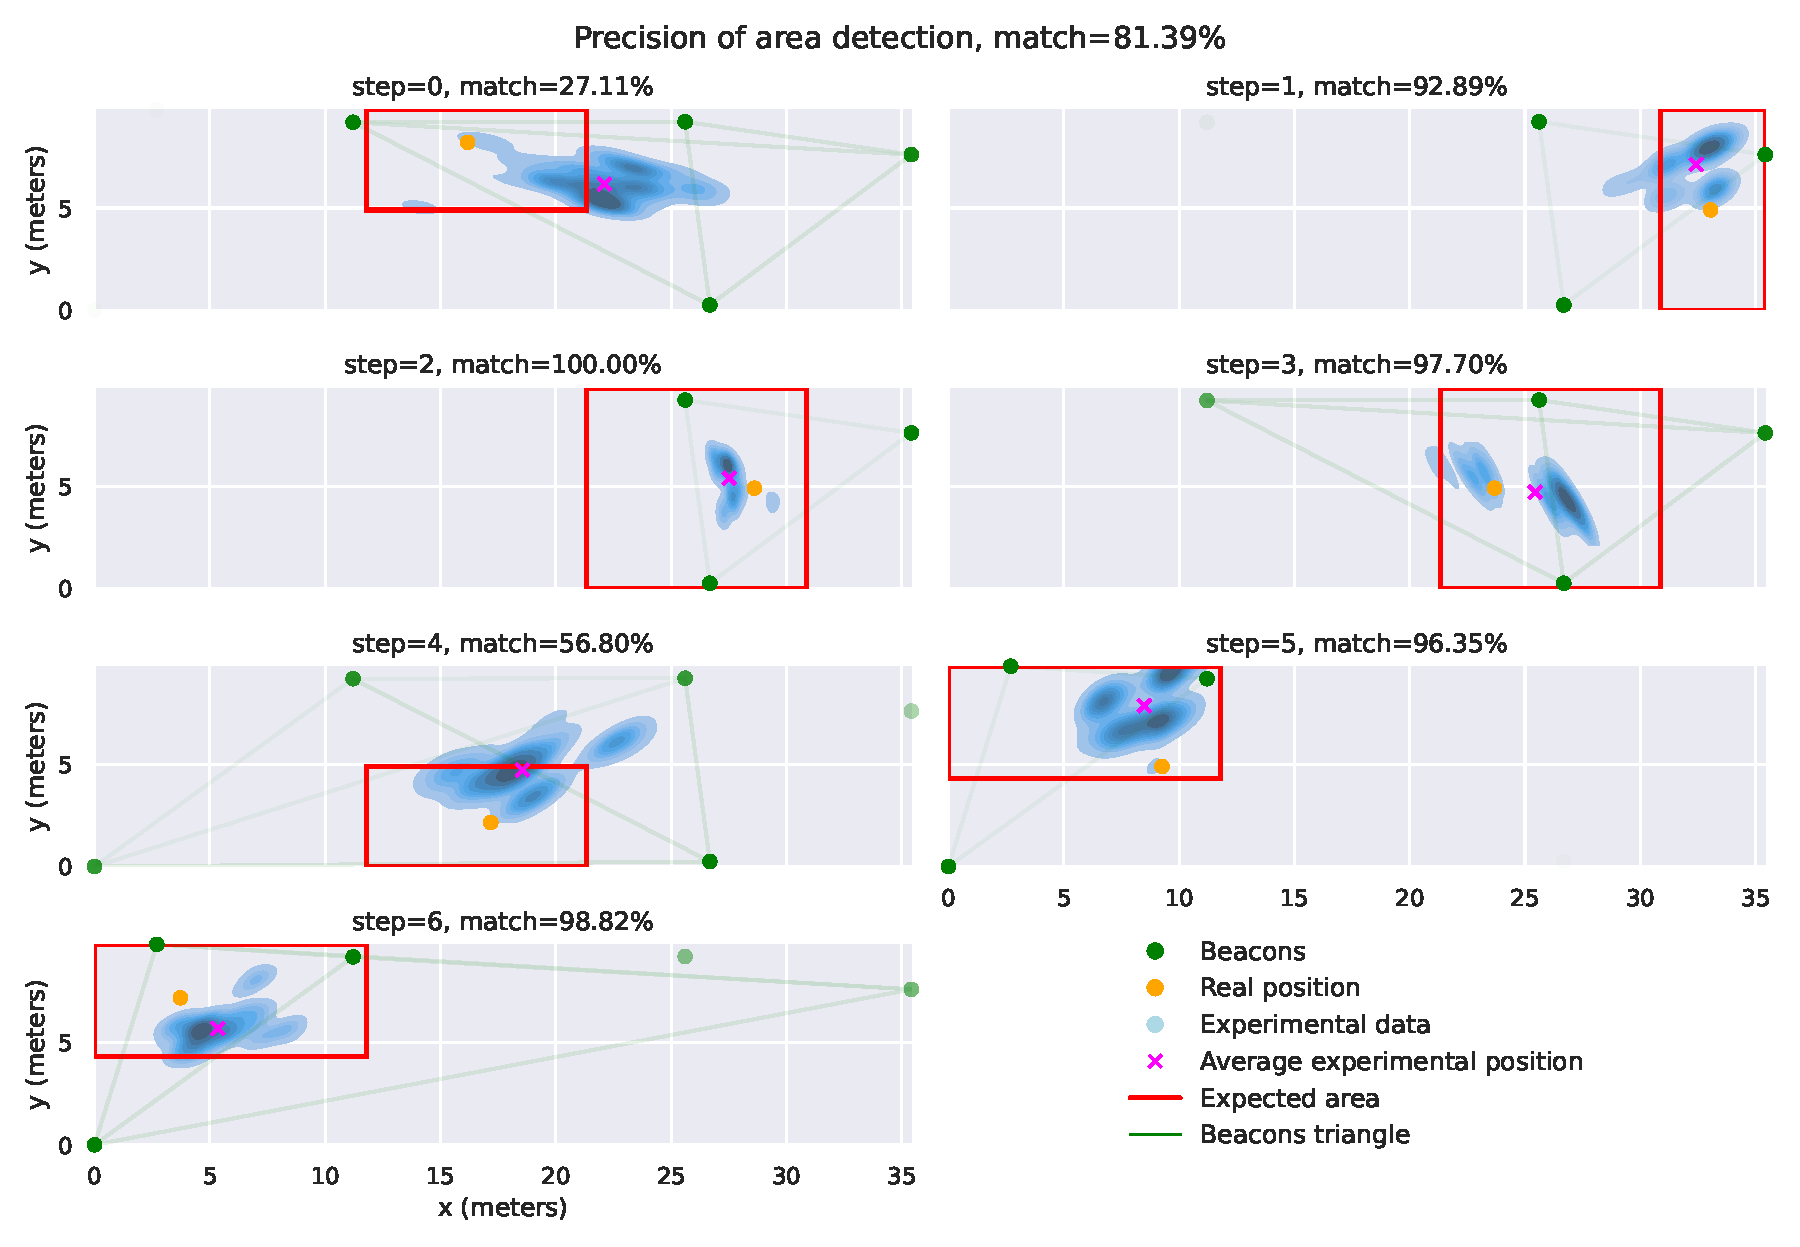
\includegraphics[width=\linewidth]{assets/museum-area-precision.pdf}
		\caption{Area detection in the museum environment}
		\label{fig:area-precision}
\end{figure}

    Several factors, including the museum's layout and the placement of beacons, may explain these discrepancies. While most of the museum floor is an open space, the central areas are divided by large stairwell walls, which can obstruct signal transmission. Moreover, as illustrated in \autoref{fig:area-precision}, the placement of the beacons is not ideal for these central zones. 

    Beacon locations are marked by green dots, with their transparency indicating the frequency of signal detection. Green triangles denote groups of three beacons used in multilateration, which are selected only if all three beacons were detected simultaneously at least 50\% of the time. In the worst-performing case (step 0), the relevant beacons are heavily off-centered from the target area, likely contributing to the low accuracy. At step 4, although up to five beacons are detected, only four are stable enough to be consistently utilized, and they typically form large, asymmetrical triangles. In contrast, better-performing steps benefit from small, well-balanced beacon triangles, which likely facilitate more accurate localization. 
     
%\section{User Experience}

\section{Summary}

This chapter presented a comprehensive evaluation of the BLE-based indoor localization system. Calibration experiments confirmed that the theoretical transmission power parameter ($tx_{power}$) is robust across environments, while the environmental factor ($N$) requires context-specific adjustment but can be applied uniformly to all beacons within a given space. Distance estimation experiments demonstrated that, after filtering, median errors in near-perfect environment can be reduced to 1.5--2.5 meters, though occasional outliers persist due to environmental noise. Multi-lateration yielded a median localization error of 2.8 meters, with the majority of position estimates falling below 4 meters of the true location, highlighting the method's reliability under typical conditions. Area detection accuracy exceeded 80\% overall, with side areas achieving near-perfect results, while central areas were more challenging due to suboptimal beacon placement and architectural obstructions. These findings underscore the importance of careful calibration and beacon deployment in achieving robust and accurate indoor localization.
